\section{External Interface Requirements}

\subsection{User Interfaces}
The user interfaces of \textit{AutomatedSOS} and \textit{Track4Run} must be intuitive and user-friendly in order to permit an easy interaction with all the services offered by the systems. The UI must be developed according to the three-click rule.\\
Moreover both the application and the web site must support multiple languages.\\
The Standard User and Special Users experiences are explained in Section \ref{userInterfaces}.

\begin{figure}[H]
\begin{minipage}{.3\textwidth}
\centering

\includegraphics[scale=.3]{img/mockup/d4h.png}
\end{minipage}
\begin{minipage}{.3\textwidth}
\centering

\includegraphics[scale=.3]{img/mockup/sos.png}
\end{minipage}
\begin{minipage}{.3\textwidth}
\centering

\includegraphics[scale=.3]{img/mockup/t4r.png}
\end{minipage}
\hspace{0.05\linewidth}
\centering
\caption{\textit{Data4Help}, \textit{AutomatedSOS} and \textit{Track4Run} logo}
\label{img:logos}
\end{figure}


\subsection{Hardware Interfaces}
The hardware interfaces of the system are huge explained in Section \ref{hardwareInterfaces}.

\subsection{Software Interfaces}
The software interfaces of the system are huge explained in Section \ref{softwareInterfaces}.

\subsection{Communication Interfaces}
The connection between clients and server and also the connection between server and payment handler must be done with the HTTPS protocol.\\
In order to manage and visualize \textit{Run}, the system must be connected with Google API to use GoogleMaps services.

\clearpage
\section{Functional Requirements}

\subsection{Individual Sign In}\label{individualLogIn}
\myparagraph{Purpose}
Anyone who wants to subscribe to one or both services offered by \textit{Data4Help} must go through the registration process, which can be carried out either through \textit{AutomatedSos} and \textit{Track4Run} apps or through the web site.
The process requires exactly the same steps regardless the platform through which it is carried out:
\begin{enumerate}
  \item The new user is required to fill in all the fields in which she/he is asked for his name, his surname, his date of birth, his city of birth, his city of residence and a valid e-mail address;
  \item The user must accept the conditions regarding his privacy, in particular the collection of his data by \textit{Data4Help} and the sharing of them in anonymous way with third parties.
\end{enumerate}
After that the system will check the correctness of the inserted data, in particular it will check that the user isn't already registerd and that the inserted e-mail isn't already used by someone else. If the result of this control is positive the registration is authorized and the user will recive a confermation e-mail to the specified e-mail address with the password she/he has to use to access to all \textit{Data4Help} services.

\myparagraph{Scenario 1}
Sara would like to register her grandmother to \textit{AutomatedSos} to not worry about her helth status when they are not together. She opens the browser on his personal computer and search for \textit{Data4Help} web site, then she clicks on the "\textit{Sign In}" button, which is located in the main page. She passes through the steps of the registration process, inserting his grandmother data and accepting the required conditions. Finally, if the inserted data are accepted by the system, she recives the confirmation e-mail.

\myparagraph{Scenario 2}
Marco wuold like to organize an amateur run with his friends and remembers that someone told him something about a new application called \textit{Track4Run} so he decides to try it. He downloads the app on his smartphone and turn it on. The first page that is shown to him contains the "\textit{Sign In}" button and the "\textit{Log In}" one, he presses on the first one and starts his registration process. He doesn't use his personal e-mail address, but an e-mail address he has in common with his brother that they usually use to make purchase online. Unexpectedly he is informed by the system that the insert e-mail is already registered in the database and so he has to change it and this time he inserts his personal e-mail address. This time the registration is succesfull and he recives the confermation e-mail.

\myparagraph{Use Case}
The Individual Sign In is analyzed in Table \ref{table:individualSignInTable}.

\myparagraph{Functional requirements}
\begin{enumerate}
  \item The system must not accept an e-mail address that is already used by an already registered user;
  \item The system must not authorize the registration untill all the fields are filled up;
  \item The system must not authorize the registration untill the required conditions aren't accepted;
  \item The system must send the confirmation e-mail to the inserted e-mail address with the password when "\textit{Submit}" button is clicked only if all the inserted data are acceptable and the required conditions has been accepted;
  \item The system must let the \textbf{Individual user to be} leave the registration process at anytime.
\end{enumerate}

\begin{center}
\begin{table}
\begin{tabular}{ | l | p{0.75\linewidth} | }
  \hline
    Actor & \textbf{Individual user to be} \\ \hline
    Goal & \textbf{[G.1]} \\ \hline
    Input Condition & A person wants to subscribe to one of \textit{Data4Help} services \\ \hline
    Event Flow & \begin{minipage}[t]{0.7\textwidth}
      \begin{enumerate}
        \item The \textbf{Individual user to be} opens the main page of \textit{Data4Help} web site from his personal computer or of \textit{AutomatedSos} or \textit{Track4Run} apps from his smartphone;
        \item The \textbf{Individual user to be} clicks on "\textit{Sign in}" button;
        \item The system shows the form the \textbf{Individual user to be} has to fill up;
        \item The \textbf{Individual user to be} fills up the form with his name, his surname, his date of birth, his city of birth, his city of residence and an e-mail address;
        \item The \textbf{Individual user to be} accepts the required conditions;
        \item The \textbf{Individual user to be} clicks on "\textit{Submit}" button;
        \item The system checks wheter the inserted information are acceptable or not;
        \item The \textbf{Individual user to be} recives a confirmation e-mail containing the password he has to use to access to all \textit{Data4Help} services.
      \end{enumerate}
    \smallskip
  \end{minipage} \\ \hline
  Output Condition & The system tells the \textbf{Individual user to be} that his registration is completed \\ \hline
  Exceptions & \begin{minipage}[t]{0.7\textwidth}
    \begin{itemize}
      \smallskip
      \item If functional requirements 1 or 2 are not satisfied the process goes back to step 4;
      \item If functional requirement 3 is not satisfied the process goes back to step 5;
      \item If the \textbf{Individual user to be} decides to leave the registration process this one is aborted.
    \end{itemize}
    \smallskip
  \end{minipage}  \\ \hline
\end{tabular}
\caption{Individual Sign In use case}
\label{table:individualSignInTable}
\end{table}
\end{center}

\clearpage

\subsection{Third Party Sign In}
\myparagraph{Purpose}
Any third party who wants to subscribe to \textit{Data4Help} must go through the registration process, which can be carried out through \textit{Data4Help} web site. The process requires several mandatory steps:
\begin{enumerate}
  \item The third party which aim to become a new member is required to fill in all the fields in which it is asked for information about the company itself like: its business name, its VAT number, its legal address, its billing address, its corporate e-mail address and the sector in which it operates;
  \item The third party must also provide the data of its legal representative, in particular his/her name, his/her surname, his/her office address, his/her phone number, his/her e-mail address and his/her SSN;
  \item The third party must select the preferred payment method;
  \item The third party must accept different conditions:
    \begin{itemize}
      \item It must assume responsibility in case of unauthorized disclosure of user data;
      \item It must accept Milan as the place of jurisdiction in the case of a legal dispute.
    \end{itemize}
\end{enumerate}
After that the system will check the correctness of the inserted data, in particular it will check that the third party isn't already registered. If the result of this control is positive the registration is authorized and the third party will receive a confirmation e-mail to the specified e-mail address with the password it has to use to access to \textit{Data4Help} services.
From now we will refer to the third party that wants to become a new member as "\textbf{Special user to Be}" to distinguish it from an Individual user.

\myparagraph{Scenario 1}
PharmaAnalisi SPA wants to acquire data of a group of young people in order to do an analysis about the kind of life they conduct. It opens the browser and search for \textit{Data4Help} web site, then it clicks on the "\textit{Third Party Sign In}" button, which is located in the main page. It passes through the steps of the registration process, inserting all the required data but forgotting to accept one of the conditions. As a consequence the system won't permit it to conclude the registration process, so it checks again and figures out what was missing, it accepts the condition and submits its registration. Finally, it receives the confimation e-mail.

\myparagraph{Use Case}
The \textit{Third Party Sign In} use case is analyzed in Table \ref{table:thirdPartySignInTable}.

\myparagraph{Mockup}
The \textit{Third Party Sign In} mocukp is shown in Figure \ref{img:thirdPartySignInMockup}.

\myparagraph{Functional requirements}
\begin{enumerate}
  \item The system must not accept an e-mail address that is already used by an already registered third party;
  \item The system must not accept a business name that is already used by an already registered third party;
  \item The system must not accept a VAT number that is already used by an already registered third party;
  \item The system must not authorize the registration untill all the fields are filled up;
  \item The system must not authorize the registration untill the preferred payment method has been selected;
  \item The system must not authorize the registration untill the required conditions aren't accepted;
  \item The system must send the confirmation e-mail to the inserted e-mail address with the password when "\textit{Submit}" button is clicked only if all the inserted data are acceptable and the required conditions has been accepted;
  \item The system must let the \textbf{Special user to be} leave the registration process at anytime.
\end{enumerate}

\begin{center}
\begin{table}
\begin{tabular}{ | l | p{0.75\linewidth} | }
  \hline
    Actor & \textbf{Special user to be} \\ \hline
    Goal & \textbf{[G.1]} \\ \hline
    Input Condition & A third party wants to subscribe to \textit{Data4Help} services \\ \hline
    Event Flow & \begin{minipage}[t]{0.7\textwidth}
      \begin{enumerate}
        \item The \textbf{Special user to be} opens the main page of \textit{Data4Help} web site.
        \item The \textbf{Special user to be} clicks on "\textit{Sign in (Third party)}" button;
        \item The system shows the form the \textbf{Special user to be} has to fill up;
        \item The \textbf{Special user to be} fills up the form with its business name, its VAT number, its legal address, its billing address, its corporate e-mail address and the sector in which it operates;
        \item The \textbf{Special user to be} selects the preferred payment method;
        \item The \textbf{Special user to be} accepts the required conditions;
        \item The \textbf{Special user to be} clicks on "\textit{Submit}" button;
        \item The system checks wheter the inserted information are acceptable or not;
        \item The \textbf{Special user to be} receives a confirmation e-mail containing the password it has to use to access to \textit{Data4Help} services.
      \end{enumerate}
    \smallskip
  \end{minipage} \\ \hline
  Output Condition & The system tells the \textbf{Special user to be} that its registration is completed \\ \hline
  Exceptions & \begin{minipage}[t]{0.7\textwidth}
    \begin{itemize}
      \smallskip
      \item If functional requirements 1,2,3 or 4 are not satisfied the process goes back to step 4;
      \item If functional requirement 5 is not satisfied the process goes back to step 5;
      \item If functional requirement 6 is not satisfied the process goes back to step 6;
      \item If the \textbf{Special user to be} decides to leave the registration process this one is aborted.
    \end{itemize}
    \smallskip
  \end{minipage}  \\ \hline
\end{tabular}
\caption{\textit{Third Party Sign In} use case}
\label{table:thirdPartySignInTable}
\end{table}
\end{center}

\begin{figure}
\begin{center}
  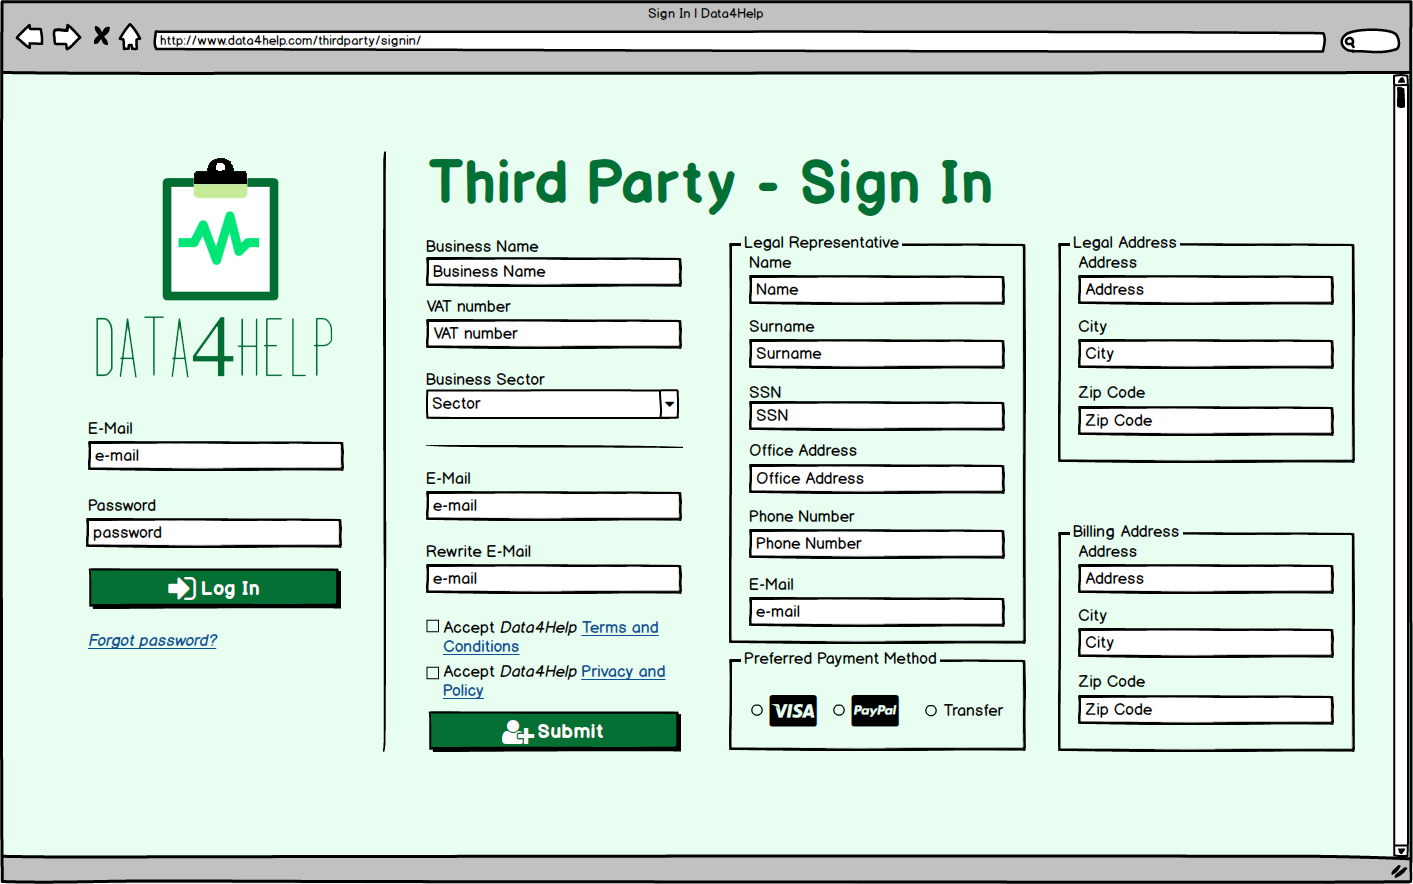
\includegraphics[width=\textwidth]{img/mockup/ThirdParty_SingIn.png}
  \hspace{0.05\linewidth}
  \centering
  \caption{\textit{Third Party Sign In} mockup}
  \label{img:thirdPartySignInMockup}
\end{center}
\end{figure}

\clearpage

\subsection{Individual Log In}
\myparagraph{Purpose}
The main goal of the login feature is to allow the access to one of the services of \textit{Data4Help} to any registered user. To access to an application the user has to fill out the credential form where e-mail and password are required. Moreover, there is a \textit{Forgot password?} section where a user could recover his/her password via e-mail. An e-mail is sended to the user with a temporary password that user will change once logged in.

\myparagraph{Scenario 1}
Francesca loves running. When she has heard about \textit{Track4Run} application she downloaded it immediately. Her friend Clara told her about a charity run for the following weekend, so Francesca opened \textit{Track4Run}, she clicked on \textit{Log in}. She inserted her e-mail address and password and clicked on the login button. Everything was correct, so she entered in the system and could enroll the run.

\myparagraph{Scenario 2}
One year ago Tommaso, Aldo's grandchild, installed on Aldo’s phone \textit{AutomatedSOS}. Yesterday, Aldo bought a new phone, he downloaded the app but he forgot his password so he couldn’t log in the application. He clicked on \textit{Forgot password?} he inserted his e-mail address and clicked on \textit{Restore my password}. He received a mail with the provisional password and he became able to access to the system. After the access he was forced to change his provisional password into a new one.

\myparagraph{Use Case}
The Individual Log In is analyzed in Table \ref{table:individualLogInInTable}.

\myparagraph{Functional requirements}
\begin{enumerate}
  \item The \textbf{Individual User} must be already registered in the system in order to log in successfully;
  \item The \textbf{Individual User} has to remember his/her e-mail address and password in order to log in successfully;
  \item The password inserted by the \textbf{Individual User} must correspond with the e-mail address;
  \item If the \textbf{Individual User} inserts wrong credential could not be able to access to the system;
  \item If the \textbf{Individual User} clicks on \textit{Forgot password?}, the system sends a new password to the \textbf{Individual User} e-mail address if and only if the e-mail address is valid and registered to the system;
  \item After a password restoring through \textit{Forgot password?} operations, the system must allow the access with the temporary password and then it has to force the \textbf{Individual User} to change the temporary password into a new one.
\end{enumerate}

\begin{center}
\begin{table}
\begin{tabular}{ | l | p{0.75\linewidth} | }
  \hline
    Actor & \textbf{Individual user} \\ \hline
    Goal & \textbf{[G.2]} \\ \hline
    Input Condition & The \textbf{Individual User} is already registered to the system and want to log in \\ \hline
    Event Flow & \begin{minipage}[t]{0.7\textwidth}
      \begin{enumerate}
        \item The \textbf{Individual User} open one of the applications (\textit{AutomatedSOS} or \textit{Track4Run});
        \item The \textbf{Individual User} clicks on \textit{Log In} button;
        \item The \textbf{Individual User} fills in the fields with his/her e-mail address and password;
        \item The \textbf{Individual User} clicks on the login button.
      \end{enumerate}
    \smallskip
  \end{minipage} \\ \hline
  Output Condition & The system allows the login of the \textbf{Individual User} and loads the dashboard of the \textbf{Individual User}. \\ \hline
  Exceptions & \begin{minipage}[t]{0.7\textwidth}
    \begin{itemize}
      \smallskip
      \item If the inserted e-mail address is never been registered to the system or the password doesn’t correspond with the email address, the system notifies the \textbf{Individual User} with an error message;
      \item If the \textbf{Individual User} inserts wrong credentials for three times the system notifies him/her with an e-mail.
    \end{itemize}
    \smallskip
  \end{minipage}  \\ \hline
\end{tabular}
\caption{Individual Log In use case}
\label{table:individualLogInInTable}
\end{table}
\end{center}

\clearpage

\subsection{Third Party Log In}
\myparagraph{Purpose}
The main goal of the login feature is to allow the access to one of the services of \textit{Data4Help} to any registered user. To access to an application the user has to fill out the credential form where e-mail and password are required. Moreover, there is a \textit{Forgot password?} section where a user could recover his/her password via e-mail. An e-mail is sended to the user with a temporary password that user will change once logged in.

\myparagraph{Scenario}
The Policlinico Cardiology Departement wants to acquire data of his/her patients, knowing their SSN.
In order to see the health status of a specific patient, Francesca - head nurse - opens her laptop and she goes to \textit{Data4Help} web site.
Francesca inserts the e-mail address of the departement and the password, the access is allowed, the system shows her the dashboard and she could be able to check her patient status.

\myparagraph{Use case and Functional Requirement}
According to the \textbf{Individual Log In} [Section \ref{individualLogIn}] functional requirements and use case are the same.\\
\textbf{Exception} is done only for the first access where device conncetion is not asked in this case.

\clearpage

\subsection{Manage Individual Profile}
\myparagraph{Purpose}
Any user can manage his personal profile both from \textit{Data4Help} web site and from \textit{AutomatedSOS} or \textit{Track4Run} applications. In particular:
\begin{itemize}
  \item The user can change some of his personal informations: his city of residence and his occupation.
  \item The user can see the data acquired on him until this moment;
  \item The user can see the past received requests about seeing his personal data;
  \item The user can see the pending received requests about seeing his personal data;
  \item The user can change his password;
  \item The user can delete his profile.
\end{itemize}

\myparagraph{Scenario 1}
Chiara has just finished her studies and has just found a new job, so she wants to update the occupation field on her profile. She opens \textit{Data4Help} web site from her personal computer, she logs in and goes in her personal area. Then she clicks on "\textit{Edit profile}" button and the system gives her the possibility to change either her city of residence or her occupation. She changes her occupation from student to emplyed and she clicks on "\textit{Submit changes}" button.

\myparagraph{Scenario 2}
Matteo has just finished the registration process, but he doesn't like the password he was given by the system and he wants to change it. He opens \textit{AutomatedSOS} application on his smartphone, logs in and accesses to his personal profile. Now he clicks on "\textit{Change password}" button and inserts the old password and the new password twice as required by the system. Finally he clicks on "\textit{Submit changes}" button.

\myparagraph{Scenario 3}
Aldo moved to USA and so he decides to delete his profile on \textit{Track4Run} because he was used to use it to organize amateur runs with his friends, but now he won't be able to do it anymore. He opens \textit{Track4Run} application on his smartphone, logs in and accesses to his personal profile. Now he clicks on "\textit{Delete profile}" button and confirm his choice. The system removes all Aldo's information from the database.

\myparagraph{Scenario 4}
CONNECT A DEVICE

\myparagraph{Use Case}
The \textit{Profile visualization} use case is analyzed in Table \ref{table:profileVisualizationTable}. \\
The \textit{Modify personal information} use case is analyzed in Table \ref{table:modifyPersonalInformationTable}. \\
The \textit{Change password} use case is analyzed in Table \ref{table:changePassowrdTable}. \\
The \textit{Delete profile} use case is analyzed in Table \ref{table:deleteProfileTable} \\

\myparagraph{Functional requirements}
\begin{enumerate}
  \item The system must let the user view his personal profile at anytime;
  \item The system must let the user upload/change his personal information at anytime;
  \item The system must let the user change his password only if the old one has been inserted correctly;
  \item The system must not let the user change his password if the new one has not been inserted twice;
  \item The system must let the user change the device connected to his profile at anytime;
  \item The system must let the user delete his profile at anytime;
  \item The system must require to confirm a deleting request;
  \item The system must not delete a profile if the choice isn't confirmed by the user;
  \item The system must let the user leave the editing profile process at anytime;
  \item The system must delete all user's personal information from its database when the user decides to delete his profile;
\end{enumerate}

\begin{center}
\begin{table}
\begin{tabular}{ | l | p{0.75\linewidth} | }
  \hline
    Actor & \textbf{User} \\ \hline
    Goal & \textbf{[G.3]} \\ \hline
    Input Condition & A \textbf{User} wants to view his personal profile\\ \hline
    Event Flow & \begin{minipage}[t]{0.7\textwidth}
      \begin{enumerate}
        \item The \textbf{User} opens \textit{Data4Help} web site or \textit{AutomatedSOS} or \textit{Track4Run} applications;
        \item The \textbf{User} logs in;
        \item The \textbf{User} accesses to his personal area;
        \item The system shows to the \textbf{User} the data acquired on him and his pending and past requests.
      \end{enumerate}
    \smallskip
  \end{minipage} \\ \hline
  Output Condition & The \textbf{User} views his personal profile with all the related information\\ \hline
  Exceptions & None \\ \hline
\end{tabular}
\caption{\textit{Profile visualization} use case}
\label{table:profileVisualizationTable}
\end{table}
\end{center}

\begin{center}
\begin{table}
\begin{tabular}{ | l | p{0.75\linewidth} | }
  \hline
    Actor & \textbf{User} \\ \hline
    Goal & \textbf{[G.3]} \\ \hline
    Input Condition & A \textbf{User} wants to modify his personal information\\ \hline
    Event Flow & \begin{minipage}[t]{0.7\textwidth}
      \begin{enumerate}
        \item The \textbf{User} opens \textit{Data4Help} web site or \textit{AutomatedSOS} or \textit{Track4Run} applications;
        \item The \textbf{User} logs in;
        \item The \textbf{User} accesses to his personal area;
        \item The \textbf{User} clicks on "\textit{Edit profile}" button;
        \item The system shows the \textbf{User} the modifiable information;
        \item The \textbf{User} modifies what he wants;
        \item The \textbf{User} click on "\textit{Submit changes}" button;
      \end{enumerate}
    \smallskip
  \end{minipage} \\ \hline
  Output Condition & The \textbf{User}'s information are modified\\ \hline
  Exceptions & \begin{minipage}[t]{0.7\textwidth}
    \begin{itemize}
      \smallskip
      \item If the \textbf{User} decides to leave the editing process this one is aborted.
    \end{itemize}
    \smallskip
  \end{minipage}  \\ \hline
\end{tabular}
\caption{\textit{Modify personal information} use case}
\label{table:modifyPersonalInformationTable}
\end{table}
\end{center}

\begin{center}
\begin{table}
\begin{tabular}{ | l | p{0.75\linewidth} | }
  \hline
    Actor & \textbf{User} \\ \hline
    Goal & \textbf{[G.3]} \\ \hline
    Input Condition & A \textbf{User} wants to change his password\\ \hline
    Event Flow & \begin{minipage}[t]{0.7\textwidth}
      \begin{enumerate}
        \item The \textbf{User} opens \textit{Data4Help} web site or \textit{AutomatedSOS} or \textit{Track4Run} applications;
        \item The \textbf{User} logs in;
        \item The \textbf{User} accesses to his personal area;
        \item The \textbf{User} clicks on "\textit{Change password}" button;
        \item The system shows the \textbf{User} the fields in which he has to insert the old and the new password;
        \item The \textbf{User} inserts the old password;
        \item The \textbf{User} inserts the new password twice;
        \item The \textbf{User} click on "\textit{Submit changes}" button;
      \end{enumerate}
    \smallskip
  \end{minipage} \\ \hline
  Output Condition & The \textbf{User}'s password is modified\\ \hline
  Exceptions & \begin{minipage}[t]{0.7\textwidth}
    \begin{itemize}
      \smallskip
      \item If functional requirement 3 is not satisfied the system goes back to step 6;
      \item If functional requirement 4 is not satisfied the system goes back to step 7;
      \item If the \textbf{User} decides to leave the editing process this one is aborted.
    \end{itemize}
    \smallskip
  \end{minipage}  \\ \hline
\end{tabular}
\caption{\textit{Change password} use case}
\label{table:changePassowrdTable}
\end{table}
\end{center}

\begin{center}
\begin{table}
\begin{tabular}{ | l | p{0.75\linewidth} | }
  \hline
    Actor & \textbf{User} \\ \hline
    Goal & \textbf{[G.3]} \\ \hline
    Input Condition & A \textbf{User} wants to delete his profile\\ \hline
    Event Flow & \begin{minipage}[t]{0.7\textwidth}
      \begin{enumerate}
        \item The \textbf{User} opens \textit{Data4Help} web site or \textit{AutomatedSOS} or \textit{Track4Run} applications;
        \item The \textbf{User} logs in;
        \item The \textbf{User} accesses to his personal area;
        \item The \textbf{User} clicks on "\textit{Delete profile}" button;
        \item The \textbf{User} confirms his choice;
      \end{enumerate}
    \smallskip
  \end{minipage} \\ \hline
  Output Condition & The \textbf{User}'s  profile is deleted\\ \hline
  Exceptions & \begin{minipage}[t]{0.7\textwidth}
    \begin{itemize}
      \smallskip
      \item If functional requirement 8 is not satisfied the deleting process is aborted;
      \item If the \textbf{User} decides to leave the deleting process this one is aborted.
    \end{itemize}
    \smallskip
  \end{minipage}  \\ \hline
\end{tabular}
\caption{\textit{Delete profile} use case}
\label{table:deleteProfileTable}
\end{table}
\end{center}

\clearpage

\subsection{Manage Third Party Profile}
\myparagraph{Purpose}
Any special user can manage its profile from \textit{Data4Help} web site, in particular:
\begin{itemize}
  \item The special user can change some of its informations: its legal address, its billing address, its corporate e-mail address and the sector in which it operates;
  \item The special user can change all the data regarding its legal representative;
  \item The special user can see the data it has required and paied until this moment;
  \item The special user can see the payments it hasn't paied yet;
  \item The special user can change the preferred payment method;
  \item The special user can change its password;
  \item The special user can delete its profile.
\end{itemize}

\myparagraph{Scenario 1}
The executive director of PincoPallo SPA had a serious fight with the legal representative of his company, and he decided to fire him a week ago. Now that he has find a new legal he wants to change the data stored in his \textit{Data4Help} profile. He accesses to \textit{Data4Help} web site from his personal pc, he logs in with the company profile and he goes in "\textit{Edit profile}" area. Now he inserts all the information about the new legal in the matching fields and then clicks on the "\textit{Submit changes}" button.

\myparagraph{Scenario 2}
AlphaAnalisi SPA wants to change the preferred payment method due to changes in its internal organization. It opens \textit{Data4Help} main page, logs in and goes in its "\textit{Edit profile}" area. It clicks on the "\textit{Change payment method}" button and selects the new preferred method. Finally it clicks on the "\textit{Submit changes}" button.

\myparagraph{Use Case}
The \textit{Special Profile Visualization} use case is analyzed in Table \ref{table:specialProfileVisualizationTable}. \\
The \textit{Modify Personal Information} use case is analyzed in Table \ref{table:modifyPersonalInformationTable}. \\
The \textit{Change Password} use case is analyzed in Table \ref{table:changePassowrdTable}. \\
The \textit{Delete Profile} use case is analyzed in Table \ref{table:deleteProfileTable}. \\

\myparagraph{Mockup}
The \textit{Special Profile Visualization} mockup is shown in Figure \ref{img:specialProfileVisualizationMockup}.

\myparagraph{Functional requirements}
\begin{enumerate}
  \item The system must let the special user view its personal profile at anytime;
  \item The system must let the special user upload/change its personal information at anytime;
  \item The system must let the special user change its password only if the old one has been inserted correctly;
  \item The system must not let the special user change its password if the new one has not been inserted correctly twice;
  \item The system must let the special user delete its profile at anytime;
  \item The system must require to confirm a deleting request;
  \item The system must not delete a profile if the choice isn't confirmed by the special user;
  \item The system must let the special user leave the editing profile process at anytime;
\end{enumerate}

\begin{center}
\begin{table}
\begin{tabular}{ | l | p{0.75\linewidth} | }
  \hline
    Actor & \textbf{Special user} \\ \hline
    Goal & \textbf{[G.3]} \\ \hline
    Input Condition & A \textbf{Special user} wants to view its profile\\ \hline
    Event Flow & \begin{minipage}[t]{0.7\textwidth}
      \begin{enumerate}
        \item The \textbf{Special user } opens \textit{Data4Help} web site;
        \item The \textbf{Special user} logs in;
        \item The \textbf{Special user} accesses to its personal area;
        \item The system shows to the \textbf{Special user} its "\textit{Edit profile}" area and the buttons to move to "\textit{Past Request}" area and "\textit{Pending Requests}" area.
      \end{enumerate}
    \smallskip
  \end{minipage} \\ \hline
  Output Condition & The \textbf{Special user} views its profile withss all the related information\\ \hline
  Exceptions & None \\ \hline
\end{tabular}
\caption{\textit{Special profile visualization} use case}
\label{table:specialProfileVisualizationTable}
\end{table}
\end{center}

\begin{figure}
\begin{center}
  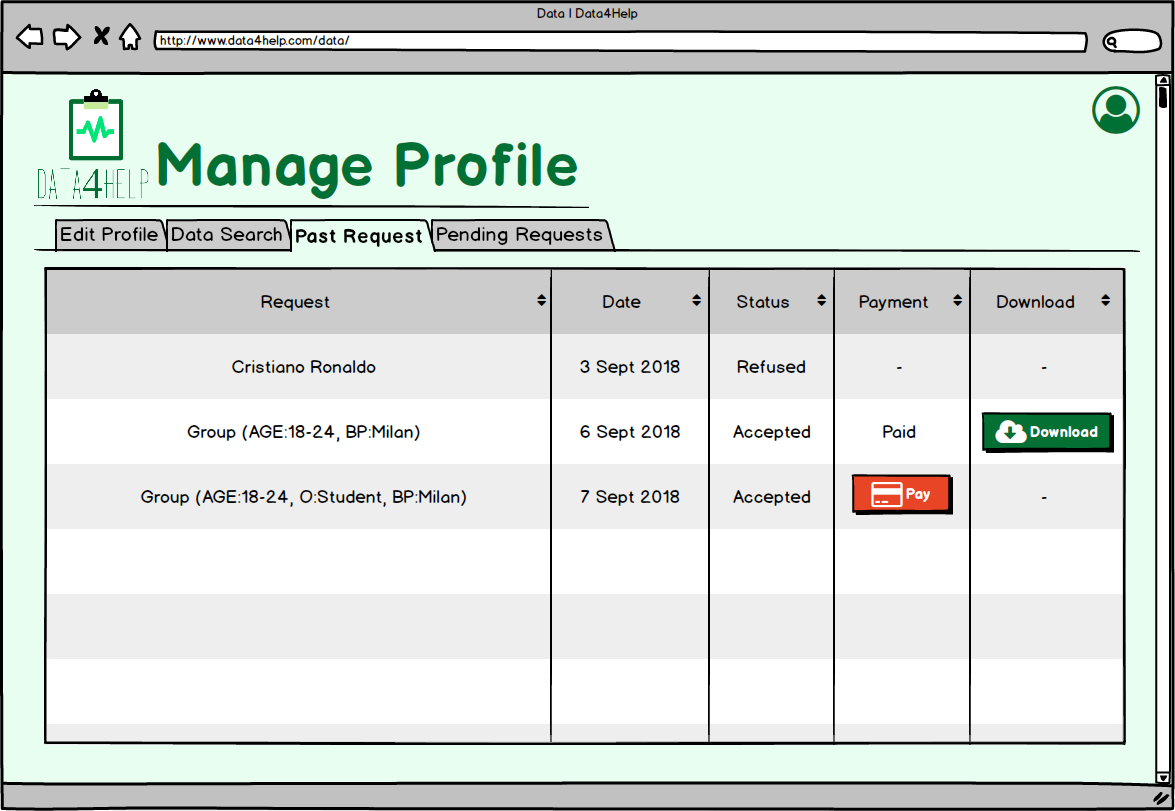
\includegraphics[width=\textwidth]{img/mockup/Searched.png}
  \hspace{0.05\linewidth}
  \centering
  \caption{\textit{Special Profile Visualization} mockup}
  \label{img:specialProfileVisualizationMockup}
\end{center}
\end{figure}

\clearpage

\subsection{Individual Data Requirement}
\myparagraph{Purpose}
Everytime a special user wants to access to the data of a specific individual it has to pass through some steps:
\begin{enumerate}
  \item It has to insert the fiscal code of the targeted individual, who will receive a direct request that he/she can accept or refuse;
  \item If the request has been accepted the special user will receive the payment form with the amount it has to pay to download the required data;
  \item If it pays the amount due it can download the required data.
\end{enumerate}

\myparagraph{Scenario 1}
AC Milan wants to acquire information about the lifestyle of Cristino Ronaldo, so it opens the browser and search for \textit{Data4Help} web site, it logs in and then it clicks on "\textit{Individual data requirement}" button. Then it inserts Ronaldo's fiscal code and waits a couple of days for a response. Unfortunately, Ronaldo doesn't accept the request and so the process ends.

\myparagraph{Scenario 2}
The "San Gerardo" hospital of Monza is trying \textit{Data4Help} combined with \textit{AutomatedSos} to monitor the health status of some of its patients after the dismissal. Lucia has been dismissed a couple of month ago and she has \textit{AutomatedSos} installed on her smartphone. The "San Gerardo" hospital accesses to \textit{Data4Help} from the web site, logs in, clicks on "\textit{Individual data requirement}" button, inserts Lucia's fiscal code and waits a couple of days for a response. Lucia accepts the request, so the "San Gerardo" hospital receives the payment form with the amount it has to pay, pays it and downloads Lucia's data.

\myparagraph{Use Case}
The Individual Data Requirement is analyzed in Table \ref{table:individualDataRequirement}.

\myparagraph{Functional requirements}
\begin{enumerate}
  \item The system must refuse a non existant fiscal code;
  \item The system must not let the special user download the required data untill it hasn't paied the amount due;
  \item The system must end the process in case of negative response from the targeted individual;
  \item The system must let the \textbf{Special user} leave the data requirement process at anytime.
\end{enumerate}

\begin{center}
\begin{table}
\begin{tabular}{ | l | p{0.75\linewidth} | }
  \hline
    Actors & \textbf{Special user} and targeted individual \\ \hline
    Goal & \textbf{[G.4]} \\ \hline
    Input Condition & A \textbf{Special user} wants to acquire data of an individual \\ \hline
    Event Flow & \begin{minipage}[t]{0.7\textwidth}
      \begin{enumerate}
        \item The \textbf{Special user} opens the main page of \textit{Data4Help} web site;
        \item The \textbf{Special user} logs in;
        \item The \textbf{Special user} click on "\textit{Individual data requirement}" button;
        \item The \textbf{Special user} inserts the fiscal code of the targeted user and waits for a response;
        \item If the response is positive the \textbf{Special user} recieves the payment form with the amount it has to pay;
        \item The \textbf{Special user} pays the amount due;
        \item The \textbf{Special user} downloads the required data.
      \end{enumerate}
    \smallskip
  \end{minipage} \\ \hline
  Output Condition & The \textbf{Special user} receives the required data \\ \hline
  Exceptions & \begin{minipage}[t]{0.7\textwidth}
    \begin{itemize}
      \smallskip
      \item If functional requirements 1 is not satisfied the process goes back to step 4;
      \item If functional requirement 2 is not satisfied the process goes back to step 6;
      \item If the targeted individual refuse to share his data the process is aborted;
      \item If the \textbf{Special user} decides to leave the data requirement process this one is aborted.
    \end{itemize}
    \smallskip
  \end{minipage}  \\ \hline
\end{tabular}
\caption{Individual Data Requirement use case}
\label{table:individualDataRequirement}
\end{table}
\end{center}

\clearpage

\subsection{Group Data Requirement}
\myparagraph{Purpose}
Everytime a special user wants to access to the data of a group of people it has to specify at least one of the required characteristics of it:
\begin{itemize}
  \item It can choose among the age ranges of the members of the targeted group proposed by the system;
  \item It can specify the Italian city of birth of the members of the targeted group;
  \item It can specify the Italian city of residence of the members of the targeted group;
  \item It can specify the Italian province of residence of the members of the targeted group;
  \item It can specify the Italian province of birth of the members of the targeted group;
  \item It can specify the Italian region of residence of the members of the targeted group;
  \item It can specify the Italian region of birth of the members of the targeted group;
  \item It can specify the state of birth of the members of the targeted group;
  \item It can specify the state of residence of the members of the targeted group;
  \item It can specify the current occupation (students, employeds, unemployeds) of the members of the targeted group.
\end{itemize}
After this the system will check if the targetd group is composed of more than 1000 people, if it is the special user will receieve the payment form with the amount it has to pay to download the required data. Once it pays the amount due it can download the required data.

\myparagraph{Scenario 1}
PharmaAnalisi SPA wants to acquire data of a group of students living in Lombardia in order to do an analysis about the kind of life they conduct. It opens the browser and search for \textit{Data4Help} web site, then it logs in and clicks on "\textit{Group data requirement}" button. It specifies that the age range of the members of the targeted group must be from 18 to 24 years old, that they should live in a city in Lombardia and that they should be students. Then it clicks on "\textit{Submit}" button and the system accepts its request, PharmaAnalisi SPA receives the payment form with the amount it has to pay, it pays the amount due and it downloads the required data.

\myparagraph{Scenario 2}
The municipality of Sondrio wants to analyze the quality of life of the people that were born in Monza and that moved to Sondrio.  It opens the browser and search for \textit{Data4Help} web site, then it logs in and clicks on "\textit{Group data requirement}" button. It specifies that the city of birth of the members of the targeted group must be Monza and that their city of residence must be Sondrio. Then it clicks on "\textit{Submit}" button but unfortunately the system tells that the required data aren't accessible because the targeted group of people is composed of less than 1000 people and so the process ends.

\myparagraph{Use Case}
The Group Data Requirement is analyzed in Table \ref{table:groupDataRequirement}.

\myparagraph{Functional requirements}
\begin{enumerate}
  \item The system must not give data of groups of people composed of less than 1000 people;
  \item The system must not let the special user download the required data untill it hasn't paid the amount due;
  \item The system must let the \textbf{Special user} leave the data requirement process at anytime.
\end{enumerate}

\begin{center}
\begin{table}
\begin{tabular}{ | l | p{0.75\linewidth} | }
  \hline
    Actor & \textbf{Special user}\\ \hline
    Goal & \textbf{[G.5]} \\ \hline
    Input Condition & A \textbf{Special user} wants to acquire data of a group of people \\ \hline
    Event Flow & \begin{minipage}[t]{0.7\textwidth}
      \begin{enumerate}
        \item The \textbf{Special user} opens the main page of \textit{Data4Help} web site;
        \item The \textbf{Special user} logs in;
        \item The \textbf{Special user} clicks on "\textit{Group data requirement}" button;
        \item The \textbf{Special user} specifies the characteristics of the targeted group;
        \item The \textbf{Special user} clicks on "\textit{Submit} button;
        \item If the targeted group is composed of more than 1000 people the \textbf{Special user} receieves the payment form with the amount it has to pay to download the required data;
        \item The \textbf{Special user} pays the amount due;
        \item The \textbf{Special user} downloads the required data.
      \end{enumerate}
    \smallskip
  \end{minipage} \\ \hline
  Output Condition & The \textbf{Special user} receives the required data \\ \hline
  Exceptions & \begin{minipage}[t]{0.7\textwidth}
    \begin{itemize}
      \smallskip
      \item If the targeted group is composed of less than 1000 people the \textbf{Special user} is informed and the process is aborted;
      \item If functional requirement 2 is not satisfied the process goes back to step 7;
      \item If the \textbf{Special user} decides to leave the data requirement process this one is aborted.
    \end{itemize}
    \smallskip
  \end{minipage}  \\ \hline
\end{tabular}
\caption{Group Data Requirement use case}
\label{table:groupDataRequirement}
\end{table}
\end{center}

\clearpage

\subsection{Health Status Visualization}
\myparagraph{Purpose}
The main feature of \textit{AutomatedSOS} is to check the health status of the user and it has to detect any critical situation.
The detection of critical situation computes a huge number of data; this computation provides several information of the health status of the user, so \textit{AutomatedSOS} provides a service to show the health status of the user.

\myparagraph{Scenario}
Silvia is worried about her grandmother because she is tired since few days. Two month ago Silvia installed on her grandmother phone \textit{AutomatedSOS} application.
In order to calm herself, Silvia takes the phone of her grandmother, she opens \textit{AutomatedSOS} and she logs in.
In the main page of the application there is the summary of the health status and everything looks ok.
To avoid any doubt Silvia clicks on the \textit{Details} button and she checks all statistics about last week and last month value of pressure and heartbeat.

\myparagraph{Use Case}
The \textit{Health Status Visualization} use case is analyzed in Table \ref{table:healthStatus}.

\myparagraph{Functional requirements}
\begin{enumerate}
  \item The system must let the user view his personal health status at anytime;
  \item The system must update the health status of the user at anytime it receives new data from the devices;
  \item The system must stores the data in order to provide monthly and weekly statustics.
\end{enumerate}

\begin{center}
\begin{table}
\begin{tabular}{ | l | p{0.75\linewidth} | }
  \hline
    Actor & \textbf{User} \\ \hline
    Goal & \textbf{[G.7]} \\ \hline
    Input Condition & A \textbf{User} wants to view his/her health status\\ \hline
    Event Flow & \begin{minipage}[t]{0.7\textwidth}
      \begin{enumerate}
        \item The \textbf{User} opens \textit{AutomatedSOS} application;
        \item The \textbf{User} logs in;
        \item The \textbf{User} accesses to \textit{My Health Status};
        \item The system shows to the \textbf{User} the data acquired on him/her with the relative computation of the health status.
      \end{enumerate}
    \smallskip
  \end{minipage} \\ \hline
  Output Condition & The \textbf{User} views his/her personal health status monitored by \textit{AutomatedSOS}\\ \hline
  Exceptions & If the system does not acquire enough data to produce statistics it notifies the \textbf{User} with a warning.  \\ \hline
\end{tabular}
\caption{\textit{Health Status Visualization} use case}
\label{table:healthStatus}
\end{table}
\end{center}

\clearpage

\subsection{Critical Situation}
\myparagraph{Purpose}
The main feature of \textit{AutomatedSOS} is to check the health status of the user and to detect any critical situation.
\textit{AutomatedSOS} monitors the health status of the subscribed customers and, when such parameters are below certain thresholds, sends to the location of the customer an ambulance, guaranteeing a reaction time of less than 5 seconds from the time the parameters are below the threshold.

\myparagraph{Scenario 1}
For a couple of days Vittorio felt very tired and affected of sickness. While he was walking in his house his heartbeat went down and he lied down on the floor. Luckily he had installed \textit{AutomatedSOS} application.
The application detected a critical situation, it managed to track Vittorio position and it called the ambulace.
The ambulace arrived very quickly and luckily the paramedics with a cardiac massage saved Vittorio that was carried to the hospital.

\myparagraph{Scenario 2}
Cristiano is a professional runner. He decides to install on his phone \textit{AutomatedSOS} to keep trace of his health status and avoid any possible critical situation when he runs.
One day, while he was running, \textit{AutomatedSOS} went in an alerted status but after only 1 second the application came back in a normal status and stayed in the normal status for all the duration of the run.
Probably it was an abnormal device measure of life value, so \textit{AutomatedSOS} did not call the ambulance.

\myparagraph{Use Case}
The \textit{Critical Situation} use case is analyzed in Table \ref{table:criticalSituation}.

\myparagraph{Mockup}
The \textit{Critical Situation} mockup is shown in Figure \ref{img:criticalSituationMockup}.

\myparagraph{Functional requirements}
\begin{enumerate}
  \item The system must guarantee a reaction time of less than 5 seconds from the time it detects an alerted situation;
  \item The system must send the location of the customer to an ambulance;
  \item The system must be in an alerted status when maximum pressure value of the customer is more than 170 mmHg and minimum pressure value is more than 100 mmHg;
  \item The system must be in an alerted status when the heartbeat is lower than 45 bmp or it is higher than 120 bpm;
  \item If the system goes in an alerted status it has to increase the life parameters detection frequency.
\end{enumerate}

\begin{center}
\begin{table}
\begin{tabular}{ | l | p{0.75\linewidth} | }
  \hline
    Actor & \textbf{User} \\ \hline
    Goal & \textbf{[G.8]} \\ \hline
    Input Condition & The system goes in an alerted status \\ \hline
    Event Flow & \begin{minipage}[t]{0.7\textwidth}
      \begin{enumerate}
        \item The system gets the GPS position of the \textbf{User};
        \item The system increases parameters detection with a frequence of 3 detection per second;
        \item The system shows an alert message on the \textbf{User}'s device (smartwatch or similar).
      \end{enumerate}
    \smallskip
  \end{minipage} \\ \hline
  Output Condition & The system calls an ambulance and it sends the location to the called ambulance if it is in an alert status from 3 seconds. \\ \hline
  Exceptions & \begin{minipage}[t]{0.7\textwidth}
    \begin{itemize}
      \smallskip
      \item If functional requirement 2 is not satisfied the system notifies the ambulance about the detected position error and sends the last detected position;
      \item If functional requirements 3 and 4 are not satisfied the system notifies the \textbf{User} with a warning message and invites the him/her to check the status and the conncetion of his/her devices.
    \end{itemize}
    \smallskip
  \end{minipage}  \\ \hline
\end{tabular}
\caption{\textit{Critical Situation} use case}
\label{table:criticalSituation}
\end{table}
\end{center}

\begin{figure}
\begin{center}
  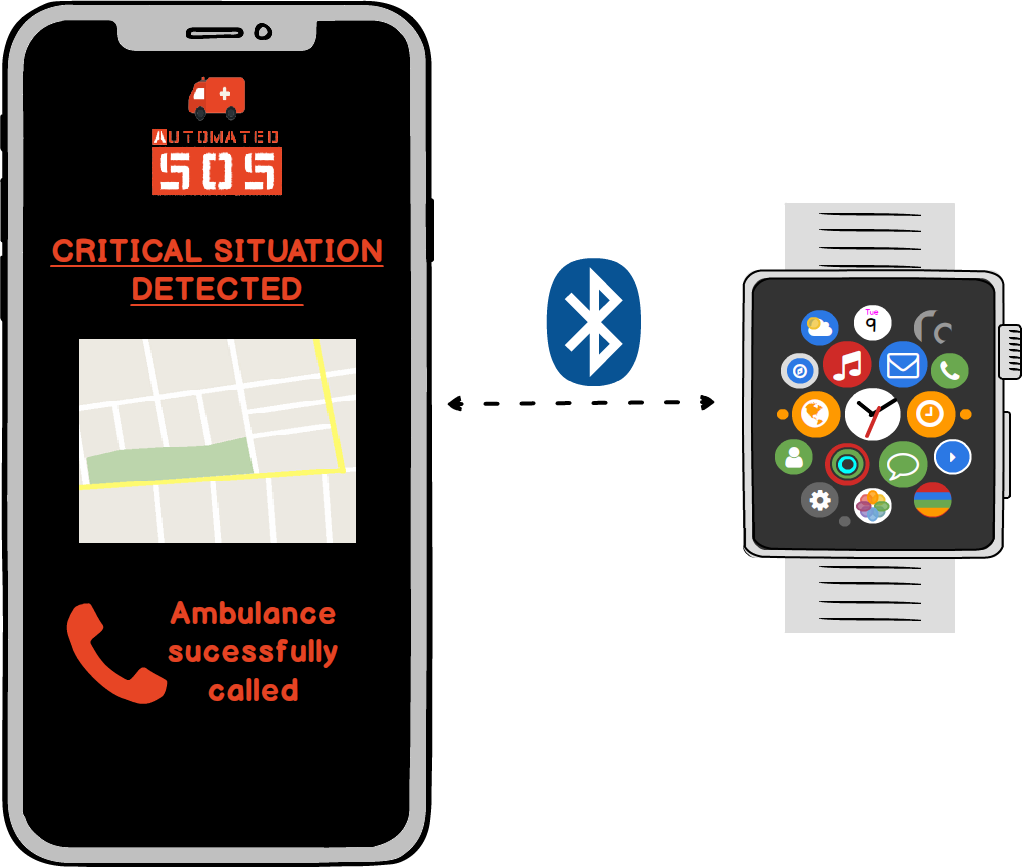
\includegraphics[width=\textwidth]{img/mockup/Critical_Situation.png}
  \hspace{0.05\linewidth}
  \centering
  \caption{\textit{Critical Situation} mockup}
  \label{img:criticalSituationMockup}
\end{center}
\end{figure}

\clearpage

\subsection{Create a Run}
\myparagraph{Purpose}
Very important feature of \textit{Track4Run} is the possibility for a \textit{Organizer} to be able to create a new \textit{Run}.
To create a \textit{Run} an \textit{Organizer} must define:
\begin{itemize}
  \item The path of the \textit{Run} through an intercative tool;
  \item The date of the \textit{Run};
  \item The maximum number of participants to the \textit{Run};
  \item The expiration date to enroll the \textit{Run};
\end{itemize}

\myparagraph{Scenario}
Massimo want to organize a charity \textit{Run} in his little town. He is already registered to \textit{Track4Run} as a Runner. After he has done all permission he goes to \textit{Track4Run} web site.
With the same credential of the mobile application he logged in the system and in the dashboard he clicked on \textit{Create a Run}. Massimo set the path trought the intercative tool, he fixed the date of the \textit{Run} and the missing fields. When everything was correct he clicked on the \textit{Create} button and the \textit{Run} went on-line.


\myparagraph{Use Case}
The \textit{Create a Run} use case is analyzed in Table \ref{table:createRunTable}.

\myparagraph{Functional requirements}
\begin{enumerate}
  \item The system must not accept \textit{Run} with date less than or equal to the current one;
  \item The system must not accept \textit{Run} with expiration date less than or equal to the current one;
  \item The system must not accept \textit{Run} with maximum nuber of participants less than or equal to 1.
  \item The system must not accept \textit{Run} with a path duplication greater or equal to the 80 percent in the same date of the new one;
\end{enumerate}

\begin{center}
\begin{table}
\begin{tabular}{ | l | p{0.75\linewidth} | }
  \hline
    Actor & \textbf{Organizer} \\ \hline
    Goal & \textbf{[G.10]} \\ \hline
    Input Condition & The \textbf{Organizer} want to create a new \textit{Run} \\ \hline
    Event Flow & \begin{minipage}[t]{0.7\textwidth}
      \begin{enumerate}
        \item The \textbf{Organizer} open \textit{Track4Run} service through web application and he/she log in;
        \item The \textbf{Organizer} clicks on \textit{Create a Run} button;
        \item The \textbf{Organizer} inserts path, date, expiration date and maximum number of participants;
        \item The \textbf{Organizer} clicks on the \textit{Create} button;
      \end{enumerate}
    \smallskip
  \end{minipage} \\ \hline
  Output Condition & The system registers the new \textit{Run} and it notifies him/her with a confirmation e-mail. \\ \hline
  Exceptions & \begin{minipage}[t]{0.7\textwidth}
    \begin{itemize}
      \smallskip
      \item If functional requirements 1, 2, 3 or 4 are not satisfied the system notifies the \textbf{Organizer} with an error message and the process goes back to step 3;
      \item In order to prevent functional requirements 4 failure, during the building phase of the path the system continuously checks satisfaction and when the functional requirement is not satisfied it notifies the \textbf{Organizer} with a warning;
      \item If the \textbf{Organizer} decides to leave the creation process this one is aborted.
    \end{itemize}
    \smallskip
  \end{minipage}  \\ \hline
\end{tabular}
\caption{\textit{Create a Run} use case}
\label{table:createRunTable}
\end{table}
\end{center}

\clearpage

\subsection{Delete a Run}
\myparagraph{Purpose}
As we have the possibilty in \textit{Track4Run} for an organizer to create a new \textit{Run}, the system must also be able to manage the decision of an organizer to delete a \textit{Run}.

\myparagraph{Scenario}
Alice wants to delete a \textit{Run} that she had organized for the next month, because the weather forecast are not optimal.
In order to avoid a rainy day Alice opened \textit{Track4Run} web-site, she logged in and she clicked on the "\textit{Manage a Run}" button.
On top of the table there was the \textit{Run} that she was looking for and she clicked on its "\textit{Delete}" button.
After that a mail arrived in Alice mailbox, it was the confirmation of the elimination of the \textit{Run}.

\myparagraph{Use Case}
The \textit{Delete A Run} use case is analyzed in Table \ref{table:deleteRunTable}.

\myparagraph{Activity Diagram}
The \textit{Delete A Run} activity diagram is shown in Figure \ref{img:deleteRunActivityDiagram}.

\myparagraph{Mockup}
The \textit{Delete A Run} mockup is shown in Figure \ref{img:deleteRunMockup}.

\myparagraph{Functional requirements}
\begin{enumerate}
  \item The system must not show \textit{Run}, in \textit{Manage a Run} section, of which an \textbf{Organizer} is not the owner;
  \item The system must let the \textbf{Organizer} leave the deletion process at anytime.
\end{enumerate}

\begin{center}
\begin{table}[H]
\begin{tabular}{ | l | p{0.75\linewidth} | }
  \hline
    Actor & \textbf{Organizer} \\ \hline
    Goal & \textbf{[G.11]} \\ \hline
    Input Condition & An \textbf{Organizer} wants to delete a \textit{Run} \\ \hline
    Event Flow & \begin{minipage}[t]{0.7\textwidth}
      \begin{enumerate}
        \item The \textbf{Organizer} opens \textit{Track4Run} service through web application and he/she logs in;
        \item The \textbf{Organizer} clicks on the "\textit{Manage a Run}" button;
        \item The \textbf{Organizer} looks for a \textit{Run} through the search bar or looking to the proposed ones;
        \item The \textbf{Organizer} clicks on the "\textit{Delete}" button of the targeted \textit{Run}.
      \end{enumerate}
    \smallskip
  \end{minipage} \\ \hline
  Output Condition & The system deletes the \textit{Run} and notifies the \textbf{Organizer} with a confirmation e-mail. Moreover the system must notify all enrolled people in the \textit{Run} with a e-mail and delete their enrolments. \\ \hline
  Exceptions & \begin{minipage}[t]{0.7\textwidth}
    \begin{itemize}
      \smallskip
      \item If the \textbf{Organizer} looks for a \textit{Run} that is not present in the system or he/she is not the owner, the system notifies the \textbf{Organizer} with a warning message;
      \item If the \textbf{Organizer} decides to leave the elimination process this one is aborted.
    \end{itemize}
    \smallskip
  \end{minipage}  \\ \hline
\end{tabular}
\caption{\textit{Delete A Run} use case}
\label{table:deleteRunTable}
\end{table}
\end{center}

\begin{figure}[H]
\begin{center}
  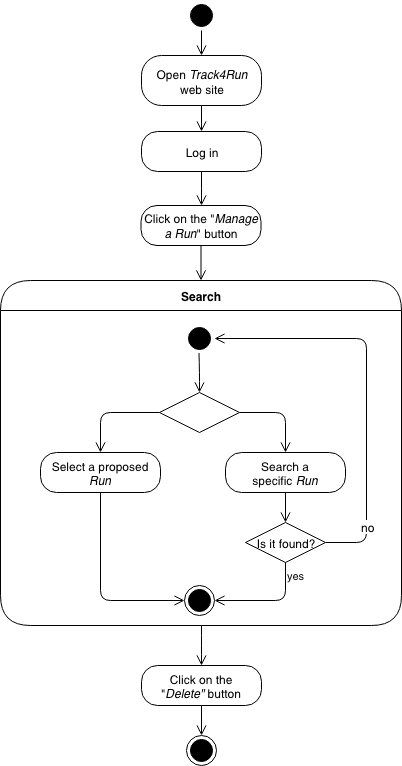
\includegraphics[height=0.6\paperheight]{img/activity/DeleteRun.png}
  \hspace{0.05\linewidth}
  \centering
  \caption{\textit{Delete A Run} activity diagram from user's point of view}
  \label{img:deleteRunActivityDiagram}
\end{center}
\end{figure}

\begin{figure}[H]
\begin{center}
  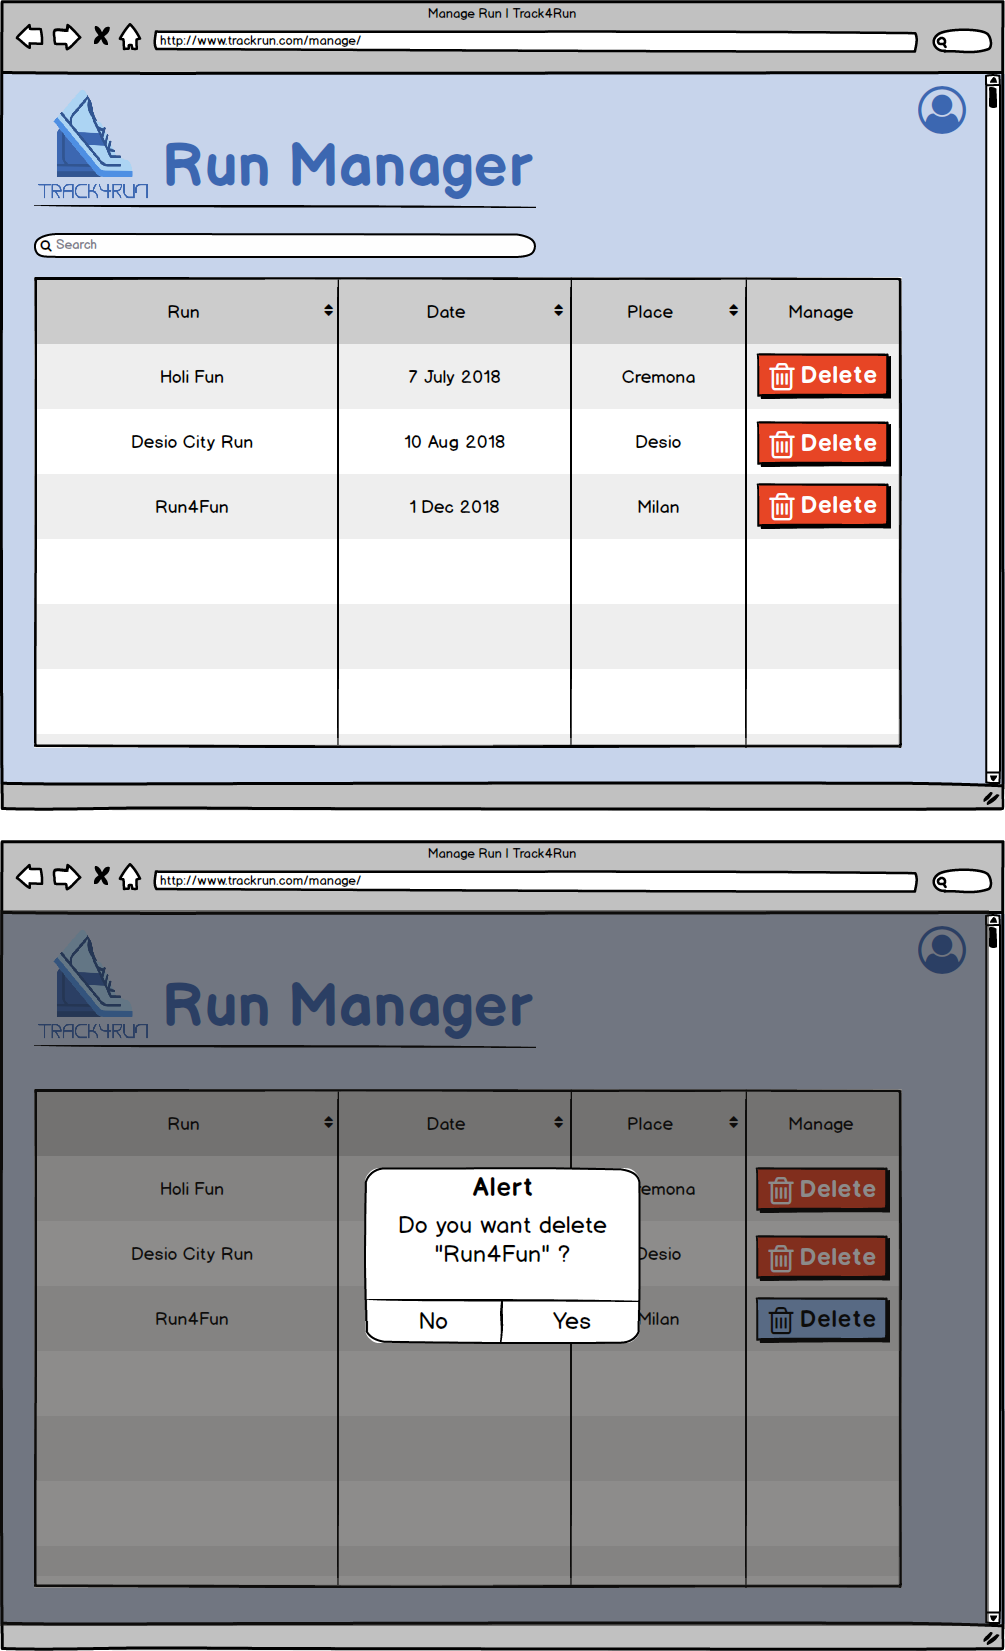
\includegraphics[height=0.6\paperheight]{img/mockup/DeleteRun.png}
  \hspace{0.05\linewidth}
  \centering
  \caption{\textit{Delete A Run} mockup}
  \label{img:deleteRunMockup}
\end{center}
\end{figure}

\clearpage

\subsection{Enrol in a Run}
\myparagraph{Purpose}
One of the great feature of \textit{Track4Run} is the possibility for a runner to be able to enrol a \textit{Run}.
In order to enrol a \textit{Run} a runner must be logged in \textit{Track4Run} application, he/she has to search the \textit{Run} that wants in the \textit{Enrol a Run} section and finally enrol it.
However, the \textit{Run} could be already done or the enrolling time expired.

\myparagraph{Scenario 1}
Andrea is technological boy. A few weeks ago he found in the Play Store the new app \textit{Track4Run} and shared his discovery with his friends. Yesterday, while he was hanging out with the buddies they discovered a new run for week-end after.
So, Andrea took his phone, he opened \textit{Track4Run} app, he logged in, he clicked on \textit{Enrol a Run} and the \textit{Run} was on top yet. So Andrea clicked on it and when the \textit{Run} event was opened he cliked on the \textit{Enrol} button.
After that Andrea received a confirmation e-mail of the correct enrolment.

\myparagraph{Scenario 2}
Samanta loves walking but for a few months now she started running. With her friend Federica she told about the city \textit{Run} planned in two day.
But unfortunately when she took her phone and opened \textit{Track4Run} she discovered that the time to enrol the \textit{Run} was expired yet.

\myparagraph{Use Case}
The \textit{Enrol a Run} use case is analyzed in Table \ref{table:enrolRunTable}.

\myparagraph{Functional requirements}
\begin{enumerate}
  \item The system must not accept an enrolment for a \textit{Run} where a \textbf{Runner} is enrolled yet.
  \item The system must not accept an enrolment for a \textit{Run} where the enrolment time is expired yet.
  \item The system must not accept an enrolment for a \textit{Run} where the maximum number of enrolment is reached;
  \item The system must not accept an enrolment for a \textit{Run} where \textbf{Runner} and \textit{Organizer} are the same person.
\end{enumerate}

\begin{center}
\begin{table}
\begin{tabular}{ | l | p{0.75\linewidth} | }
  \hline
    Actor & \textbf{Runner} \\ \hline
    Goal & \textbf{[G.12]} \\ \hline
    Input Condition & The \textbf{Runner} want to enrol a \textit{Run} \\ \hline
    Event Flow & \begin{minipage}[t]{0.7\textwidth}
      \begin{enumerate}
        \item The \textbf{Runner} open \textit{Track4Run} service through mobile application and he/she log in;
        \item The \textbf{Runner} clicks on \textit{Enrol a Run} button;
        \item The \textbf{Runner} looks for a \textit{Run} through the search bar or looking to the proposed;
        \item The \textbf{Runner} clicks on the \textit{Run} he/she wants to enrol;
        \item The \textbf{Runner} clicks on the \textit{Enrol}.
      \end{enumerate}
    \smallskip
  \end{minipage} \\ \hline
  Output Condition & The system registers the enrolment of the \textbf{Runner} and it notifies him/her with a confirmation e-mail. \\ \hline
  Exceptions & \begin{minipage}[t]{0.7\textwidth}
    \begin{itemize}
      \smallskip
      \item If functional requirements 1, 2, 3 or 4 are not satisfied the system notifies the \textbf{Runner} with an error message and the process goes back to step 3;
      \item The \textbf{Runner} looks for a \textit{Run} that is not present in the system, the system notifies the \textbf{Runner} with a warning message;
      \item If the \textbf{Runner} decides to leave the enrolment process this one is aborted.
    \end{itemize}
    \smallskip
  \end{minipage}  \\ \hline
\end{tabular}
\caption{\textit{Enrol a Run} use case}
\label{table:enrolRunTable}
\end{table}
\end{center}

\clearpage

\subsection{Delete an Enrolment in a Run}
\myparagraph{Purpose}
As we have the possibilty in \textit{Track4Run} for a runner to be able to enrol in a \textit{Run}, the system must also be able to manage the decision of a runner to delete his/her enrolment.

\myparagraph{Scenario}
Giulia is enrolled in the annual \textit{Run} of her neighborhood. The enrolment management was made through \textit{Track4Run} application. Unfortunately for the day of the \textit{Run} Giulia will be in Florence for an important work meeting.
When Giulia received the meeting mail she took her phone, she opened \textit{Track4Run} app and she clicked on "\textit{Enrolled Run}" button.
The only row in the table was the annual \textit{Run}, Giulia clicked on it and then clicked on "\textit{Delete Enrolment}" button.
After that Giulia received a confirmation e-mail.

\myparagraph{Use Case}
The \textit{Delete An Enrolment In A Run} use case is analyzed in Table \ref{table:deleteEnrolmentTable}.

\myparagraph{Mockup}
The \textit{Delete An Enrolment In A Run} mockup is shown in Figure \ref{img:deleteEnrolmentMockup}.

\myparagraph{Functional requirements}
\begin{enumerate}
  \item The system must not show \textit{Run}, in \textit{Enrolled Run} section, in which a \textbf{Runner} is not enrolled;
  \item The system must let the \textbf{Runner} delete his/her enrolment in a \textit{Run} at anytime;
  \item The system must let the \textbf{Runner} leave the elimination process at anytime.
\end{enumerate}

\begin{center}
\begin{table}
\begin{tabular}{ | l | p{0.75\linewidth} | }
  \hline
    Actor & \textbf{Runner} \\ \hline
    Goal & \textbf{[G.13]} \\ \hline
    Input Condition & A \textbf{Runner} wants to delete an enrolment in a \textit{Run} \\ \hline
    Event Flow & \begin{minipage}[t]{0.7\textwidth}
      \begin{enumerate}
        \item The \textbf{Runner} opens \textit{Track4Run} service through mobile application and he/she logs in;
        \item The \textbf{Runner} clicks on the "\textit{Enrolled Run}" button;
        \item The \textbf{Runner} looks for a \textit{Run} through the search bar or looking to the proposed ones;
        \item The \textbf{Runner} clicks on the \textit{Run} in which he/she wants to delete the enrolment;
        \item The \textbf{Runner} clicks on the "\textit{Delete Enrolment}" button.
      \end{enumerate}
    \smallskip
  \end{minipage} \\ \hline
  Output Condition & The system deletes the enrolment of the \textbf{Runner} and it notifies him/her with a confirmation e-mail. \\ \hline
  Exceptions & \begin{minipage}[t]{0.7\textwidth}
    \begin{itemize}
      \smallskip
      \item If the \textbf{Runner} looks for a \textit{Run} that is not present in the system, the system notifies the \textbf{Runner} with a warning message;
      \item If the \textbf{Runner} decides to leave the elimination process this one is aborted.
    \end{itemize}
    \smallskip
  \end{minipage}  \\ \hline
\end{tabular}
\caption{\textit{Delete An Enrolment In A Run} use case}
\label{table:deleteEnrolmentTable}
\end{table}
\end{center}

\begin{figure}
\begin{center}
  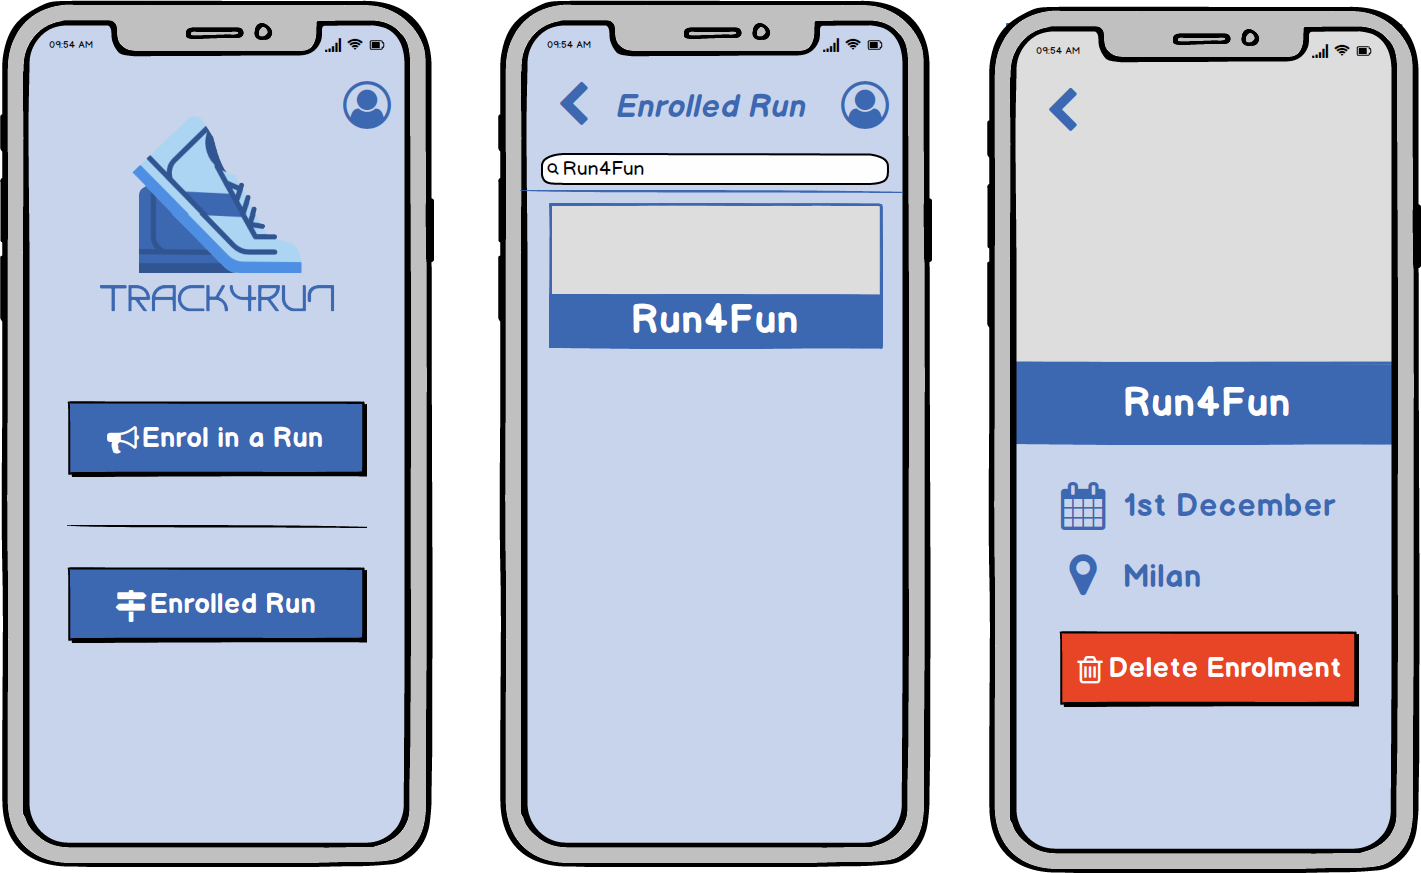
\includegraphics[width=\textwidth]{img/mockup/DeleteEnrolment.png}
  \hspace{0.05\linewidth}
  \centering
  \caption{\textit{Delete An Enrolment In A Run} mockup}
  \label{img:deleteEnrolmentMockup}
\end{center}
\end{figure}

\clearpage

\subsection{Run Watching}
\myparagraph{Purpose}
For each \textit{Run}, that is present in the system, a \textit{Specator} or an \textit{User} must be able to watch it. The \textit{Spectator} or the \textit{User} could follow the positon, on the \textit{Run} path, of any person that has enroled the \textit{Run} and also he/she must be able to look at the placing table of the runners.

\myparagraph{Scenario 1}
Marco is a professional runner and play for a team, unfortunately one month ago he broke his leg. Today there is an important \textit{Run} and his teammates are enrolled. At 4 p.m., Marco will open \textit{Track4Run} app on his mobile phone, in the dashboard he will look for the today's \textit{Run}, he will click on it and immediately he will be "in the \textit{Run}"; he could follow his friend on the path (watching the position on the map) and clicking on the \textit{Placings} button he could see the current placing table.

\myparagraph{Scenario 2}
Andrea is a sport event planner. With his coworker Luca, they planned the "HOLI FUN Run" of the 7\textsuperscript{th} of July in Cremona. In the \textit{Run}'s day, Andrea was in France for a meeting so when the meeting ends he went back to his hotel, he opend his laptop and he went to \textit{Track4Run} web page, he searched, through the search bar, the \textit{Run} that unfortunately was just ended, however he was very happy because looking at the placing table he saw that his friend Marta won.

\myparagraph{Use Case}
The Run Watching is analyzed in Table \ref{table:visitRunTable}.

\myparagraph{Functional requirements}
\begin{enumerate}
  \item \textbf{Generic User} (that could be \textit{Specator} or \textit{User}) must be able to watch a \textit{Run} that is still in progress or ended;
  \item The system must continuously check the positon of the runner in order to keep the map and the placing table updated;
  \item The system must be able to show all the runners that enroled the \textit{Run} and their GPS position is enabled and nearby the path;
  \item The system must notify the end of a \textit{Run} to a \textbf{Specator} or an \textbf{User} that is watching it;
  \item The system must be able to compute the placing table through the GPS position of the runner enroled in the \textit{Run}.
\end{enumerate}

\begin{center}
\begin{table}
\begin{tabular}{ | l | p{0.75\linewidth} | }
  \hline
    Actor & \textbf{Generic User} that could be \textit{Specator} or \textit{User} \\ \hline
    Goal & \textbf{[G.13]} \\ \hline
    Input Condition & The \textbf{Generic User} want to watch a \textit{Run} \\ \hline
    Event Flow & \begin{minipage}[t]{0.7\textwidth}
      \begin{enumerate}
        \item The \textbf{Generic User} open \textit{Track4Run} service through mobile application or web application;
        \item The \textbf{Generic User} clicks on \textit{Watch a Run} button;
        \item The \textbf{Generic User} looks for a \textit{Run} through the search bar or looking to the proposed;
        \item The \textbf{Generic User} clicks on the \textit{Run} he/she wants to watch.
      \end{enumerate}
    \smallskip
  \end{minipage} \\ \hline
  Output Condition & The system loads the \textit{Run} environment (map, path and placing table) and  shows it to the \textbf{Generic User}. \\ \hline
  Exceptions & \begin{minipage}[t]{0.7\textwidth}
    \begin{itemize}
      \smallskip
      \item The \textbf{Generic User} looks for a \textit{Run} that is not present in the system, the system notifies the \textbf{Generic User} with a warning message;
      \item If the connection of the \textbf{Generic User} application is lost and the system couldn't be able to recover it the process goes back to step 3.
    \end{itemize}
    \smallskip
  \end{minipage}  \\ \hline
\end{tabular}
\caption{Run Watching use case}
\label{table:visitRunTable}
\end{table}
\end{center}

\clearpage
